\documentclass[12pt]{article}
\usepackage{graphicx}
\usepackage{amsmath}
\usepackage{amssymb}
\usepackage{hyperref}
\usepackage{geometry}
\usepackage{float}
\usepackage{booktabs}
\usepackage{listings}
\usepackage{xcolor}
\usepackage{tikz}
\usetikzlibrary{positioning}
\geometry{margin=1in}

\lstset{
  language=Python,
  basicstyle=\small\ttfamily,
  keywordstyle=\color{blue},
  commentstyle=\color{gray},
  stringstyle=\color{red},
  frame=single,
  breaklines=true,
  numbers=left,
  numberstyle=\tiny\color{gray},
  showstringspaces=false
}

\title{Active Learning Strategies for Label Propagation on Graphs}
\author{Jamey Harris}
\date{April 2026}

\begin{document}

\maketitle

\begin{abstract}
In many application domains, obtaining labeled data is expensive and time-consuming, motivating methods that can leverage small labeled sets to classify large unlabeled datasets. Graph-based semi-supervised learning addresses this by propagating labels through a similarity graph. The Gaussian Fields and Harmonic Functions (GFHF) method \cite{Zhu2003} computes a harmonic function over the graph that smoothly interpolates known labels to unlabeled nodes. However, GFHF does not specify \textit{which} nodes should be labeled. This project investigates how active learning query strategies affect GFHF classification accuracy under limited labeling budgets and noisy conditions. Four strategies are compared --- random selection, uncertainty sampling \cite{Lewis1994}, maximum weighted degree, and betweenness centrality \cite{Freeman1977} --- across three synthetic datasets and four noise levels. Results show that uncertainty sampling consistently outperforms all alternatives, while maximum degree selection performs worse than random on datasets with non-trivial decision boundaries. These findings demonstrate that targeting nodes at class boundaries is more effective than targeting structurally prominent nodes for graph-based label propagation.
\end{abstract}

%==============================================================================
\section{Introduction}
%==============================================================================

In many application domains, obtaining labeled data can be resource-intensive, time-consuming, and may require specialized expert knowledge. Protein crystallography, for example, can cost upwards of \$270,000 to determine the shape of a single protein \cite{Zhu2003}. Cybersecurity threat classification demands analysts who can distinguish between benign and malicious network activity. Document classification at scale requires subject-matter experts familiar with the taxonomy being applied \cite{Bilgic2010}. In these domains, only a small subset of data points can feasibly be labeled within practical time and cost constraints. This limitation motivates the development of machine learning methods that can leverage a small set of labeled data points to infer labels for the remaining unlabeled data, greatly reducing the resources required \cite{Chapelle2006}.

One approach to propagating labels across a dataset with few labeled data points is graph-based semi-supervised learning \cite{Zhu2005}. By framing the data as a graph where data points are represented as vertices, we can encode the similarity between data points as weighted edges. Under the \textit{smoothness assumption} --- the principle that nearby or strongly connected nodes in the graph are likely to share the same label \cite{Chapelle2006, Zhu2005} --- labels assigned to a small subset of nodes can be propagated to the remaining unlabeled nodes through the graph structure.

A foundational approach in this setting is the Gaussian Fields and Harmonic Functions (GFHF) method, introduced by Zhu, Ghahramani, and Lafferty \cite{Zhu2003}. GFHF models the label assignment as a real-valued function over the graph and computes the unique harmonic function that minimizes a quadratic energy functional, subject to the constraint that the function agrees with the known labels on the labeled nodes. The resulting function is smooth over the graph, meaning that connected nodes with high edge weight tend to receive similar predicted values.

While GFHF is effective at propagating labels from a small labeled subset, it does not address \textit{which} nodes should be labeled in the first place. The choice of which nodes to label can have a significant impact on classification accuracy. This observation motivates the integration of \textit{active learning} strategies, which aim to select the most informative nodes to query for labels under a fixed labeling budget $B$ \cite{Settles2012}. This project investigates how different active learning query strategies affect the accuracy of GFHF-based label propagation and how robust these strategies are under noisy labeling conditions where queried labels may be incorrect.

\subsection{Key Definitions}

The following definitions establish the terminology used throughout this paper.

\textbf{Graph.} A graph $G = (V, E)$ consists of a set of vertices (or nodes) $V$ and a set of edges $E \subseteq V \times V$ connecting pairs of vertices. Graphs model pairwise relationships between objects \cite{Diestel2017}.

\textbf{Weighted Graph.} A weighted graph $G = (V, E, W)$ augments a graph with a weight function $W: E \rightarrow \mathbb{R}^+$ that assigns a non-negative real value to each edge. In graph-based semi-supervised learning, edge weights encode the similarity between data points: a larger weight $w_{ij}$ indicates that nodes $i$ and $j$ are more similar \cite{Zhu2003}.

\textbf{Labeled and Unlabeled Sets.} The vertex set $V$ is partitioned into a labeled set $L$ and an unlabeled set $U = V \setminus L$, where $|L| = l \ll n = |V|$. Each labeled node $i \in L$ has a known class label $y_i \in \{0, 1\}$.

\textbf{Harmonic Function.} A function $f: V \rightarrow \mathbb{R}$ is harmonic on $U$ if, for every unlabeled node $j \in U$, the value $f(j)$ equals the weighted average of $f$ over the neighbors of $j$ \cite{Zhu2003}. Harmonic functions arise naturally as the solutions that minimize the graph smoothness energy.

\textbf{Active Learning.} Active learning is a machine learning paradigm in which the learning algorithm can interactively query an oracle (e.g., a human annotator) for labels of selected data points, rather than passively receiving a fixed labeled training set \cite{Settles2012}. The goal is to achieve high accuracy with as few labeled examples as possible by strategically choosing which instances to label.

\textbf{Label Propagation.} Label propagation refers to the process of inferring labels for unlabeled nodes in a graph by spreading information from labeled nodes through the graph structure, guided by edge weights \cite{Zhu2005}.


%==============================================================================
\section{Background and Literature}
%==============================================================================

\subsection{Gaussian Fields and Harmonic Functions}

Zhu, Ghahramani, and Lafferty \cite{Zhu2003} introduced the Gaussian Fields and Harmonic Functions (GFHF) method, establishing a foundational technique in graph-based semi-supervised learning. The approach begins by constructing a graph where every data point is a node, and edges connect nodes that are similar. The edges are weighted so that more similar nodes receive stronger connections. A common way to measure this similarity is the Gaussian kernel: the closer two points are in feature space, the higher their edge weight, and the weight drops off exponentially as distance increases \cite{Zhu2003}. A parameter $\sigma$ controls the rate of this decay --- small $\sigma$ means only very nearby points are considered similar, while large $\sigma$ allows more distant points to retain significant edge weight.

The central idea of GFHF is that each unlabeled node's predicted value should equal the \textit{weighted average of its neighbors' values} \cite{Zhu2003}. If most of a node's neighbors lean toward class 1, that node is likely class 1 as well. The algorithm proceeds as follows:

\begin{enumerate}

\item \textbf{Weighted Graph Construction.}
Begin with a weighted graph $G = (V, E)$ where each of the $n$ data points corresponds to a node. Edge weights $w_{ij}$ encode the similarity between data points $i$ and $j$ \cite{Zhu2003}.

\item \textbf{Gaussian Kernel.}
Edge weights are computed using the Gaussian (radial basis function) kernel \cite{Zhu2003}:
\[
w_{ij} = \exp\!\left(-\frac{\|x_i - x_j\|^2}{2\sigma^2}\right),
\]
where $\sigma$ is a length-scale hyperparameter. The first $l$ nodes are labeled with known values $f_l = (y_1, \ldots, y_l)$, and the remaining $u = n - l$ nodes are unlabeled.

\item \textbf{Harmonic Function.}
GFHF computes a harmonic function $f$ over the graph that satisfies the averaging property: for each unlabeled node $j$ \cite{Zhu2003},
\[
f(j) = \frac{1}{d_j} \sum_{i \sim j} w_{ij}\, f(i),
\]
where $d_j = \sum_{i} w_{ij}$ is the weighted degree of node $j$. This leads to the closed-form solution for the unlabeled nodes:
\[
f_u = (D_{uu} - W_{uu})^{-1}\, W_{ul}\, f_l.
\]

\item \textbf{Energy Minimization.}
The harmonic function equivalently minimizes the graph smoothness energy \cite{Zhu2003}:
\[
E(f) = \frac{1}{2} \sum_{i,j} w_{ij}\,(f(i) - f(j))^2,
\]
subject to labeled nodes remaining fixed. Minimizing this energy ensures that nodes connected by strong edges receive similar predicted values. This energy functional is closely related to the combinatorial graph Laplacian $\Delta = D - W$ \cite{Zhu2003}.

\item \textbf{Matrix Definitions.}
In the closed-form solution:
\begin{itemize}
\item $D_{uu}$ is the diagonal degree matrix restricted to unlabeled nodes, where each diagonal entry is the total edge weight from that unlabeled node to all other nodes.
\item $W_{uu}$ is the weight submatrix capturing connections among unlabeled nodes.
\item $W_{ul}$ is the weight submatrix capturing connections from unlabeled nodes to labeled nodes.
\item $(D_{uu} - W_{uu})$ is the graph Laplacian restricted to the unlabeled nodes \cite{Zhu2003}.
\end{itemize}

\end{enumerate}

\subsection{Worked Example: GFHF on a Small Graph}

To build intuition for the GFHF method, consider a small graph with five nodes as shown in Figure~\ref{fig:toy_graph}. Nodes 1 and 5 are labeled: $y_1 = 1$ (class 1) and $y_5 = 0$ (class 0). Nodes 2, 3, and 4 are unlabeled.

\begin{figure}[H]
\centering
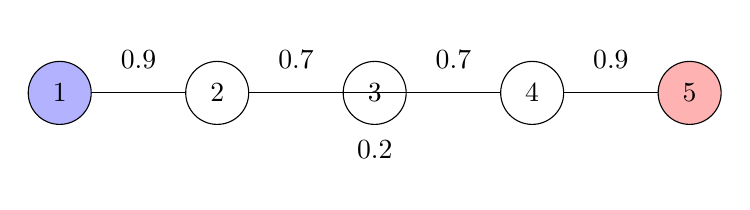
\begin{tikzpicture}[node distance=2cm, every node/.style={circle, draw, minimum size=0.8cm}]
  \node[fill=blue!30] (1) {1};
  \node[right of=1] (2) {2};
  \node[right of=2] (3) {3};
  \node[right of=3] (4) {4};
  \node[right of=4, fill=red!30] (5) {5};

  \draw (1) -- node[above, draw=none, minimum size=0] {0.9} (2);
  \draw (2) -- node[above, draw=none, minimum size=0] {0.7} (3);
  \draw (3) -- node[above, draw=none, minimum size=0] {0.7} (4);
  \draw (4) -- node[above, draw=none, minimum size=0] {0.9} (5);
  \draw (2) -- node[below, draw=none, minimum size=0, yshift=-0.3cm] {0.2} (4);
\end{tikzpicture}
\caption{A small graph with 5 nodes. Nodes 1 (blue, $y_1=1$) and 5 (red, $y_5=0$) are labeled. Edge weights reflect similarity. The GFHF harmonic function must satisfy the averaging property at unlabeled nodes 2, 3, and 4.}
\label{fig:toy_graph}
\end{figure}

The labeled set is $L = \{1, 5\}$ with labels $f_l = (1, 0)^T$, and the unlabeled set is $U = \{2, 3, 4\}$. From the edge weights, the relevant submatrices are:
\[
W_{uu} = \begin{pmatrix} 0 & 0.7 & 0.2 \\ 0.7 & 0 & 0.7 \\ 0.2 & 0.7 & 0 \end{pmatrix}, \quad
W_{ul} = \begin{pmatrix} 0.9 & 0 \\ 0 & 0 \\ 0 & 0.9 \end{pmatrix}.
\]
The degree matrix for unlabeled nodes sums all weights from each unlabeled node (including connections to labeled nodes):
\[
D_{uu} = \begin{pmatrix} 1.8 & 0 & 0 \\ 0 & 1.4 & 0 \\ 0 & 0 & 1.8 \end{pmatrix}.
\]
The graph Laplacian restricted to unlabeled nodes is $A = D_{uu} - W_{uu}$, and the right-hand side is $b = W_{ul} f_l$:
\[
A = \begin{pmatrix} 1.8 & -0.7 & -0.2 \\ -0.7 & 1.4 & -0.7 \\ -0.2 & -0.7 & 1.8 \end{pmatrix}, \quad
b = \begin{pmatrix} 0.9 \\ 0 \\ 0 \end{pmatrix}.
\]
Solving $A f_u = b$ yields approximately $f_u = (0.72,\; 0.50,\; 0.28)^T$. The predictions are interpretable: node~2, which is close to the class-1 label, receives $f(2) \approx 0.72$ (classified as class 1). Node~4, which is close to the class-0 label, receives $f(4) \approx 0.28$ (classified as class 0). Node~3, equidistant from both labeled nodes, receives $f(3) \approx 0.50$ --- maximal uncertainty, sitting exactly at the decision boundary. Under the simple thresholding rule ($\hat{y}_i = 1$ if $f(i) \geq 0.5$), node~3 would be classified as class~1, though the confidence is minimal.

This example illustrates why uncertainty sampling would select node~3 for labeling: it is the node where the model is least confident, and resolving its true label would provide the most information about where the decision boundary lies.

\subsection{Class Mass Normalization}

A straightforward decision rule assigns label 1 to node $i$ if $f(i) > 0.5$ and label 0 otherwise. However, Zhu et al.\ \cite{Zhu2003} observed that this simple threshold can produce severely imbalanced predictions when the graph structure does not reflect the true class proportions. For instance, if one class occupies a denser region of the graph, the raw harmonic function values may be skewed toward that class, causing the majority of nodes to be assigned the same label.

Class Mass Normalization (CMN) addresses this by adjusting the decision threshold so that the predicted class proportions match the known or estimated class priors \cite{Zhu2003}. Let $q$ denote the prior probability of class 1 and $(1-q)$ the prior of class 0. Under CMN, node $i$ is classified as class 1 if and only if:
\[
\frac{q \cdot f_u(i)}{\sum_{i} f_u(i)}
\;>\;
\frac{(1-q)\,(1 - f_u(i))}{\sum_{i} (1 - f_u(i))}.
\]
This can be understood as adjusting the threshold so that the right proportion of nodes are assigned to each class. Zhu et al.\ \cite{Zhu2003} demonstrate that CMN significantly improves accuracy on digit classification and text categorization tasks where the simple threshold rule fails due to class imbalance.

\subsection{Learning Weight Function Hyperparameters}

The performance of GFHF depends on the choice of the length-scale parameter $\sigma$ in the Gaussian kernel. Zhu et al.\ \cite{Zhu2003} propose learning $\sigma$ from the data by minimizing the average label entropy:
\[
H(f) = \frac{1}{u}\sum_{i=l+1}^{l+u} H_i(f(i)),
\]
where the entropy of each unlabeled node's prediction is:
\[
H_i(f(i)) = -f(i)\,\log f(i) - (1-f(i))\,\log(1-f(i)).
\]
Low entropy indicates confident predictions --- values close to 0 or 1 rather than near 0.5. By choosing $\sigma$ to minimize this average entropy, the algorithm selects the length scale that produces the most confident labeling \cite{Zhu2003}. This entropy minimization also acts as a form of feature selection: in high-dimensional data, the algorithm can learn a separate $\sigma_d$ for each dimension, effectively identifying which dimensions are most relevant by driving irrelevant dimensions' $\sigma$ values toward infinity \cite{Zhu2003}.

\subsection{Active Learning}

Active learning is a paradigm in which the learning algorithm can interactively select which data points to query for labels, rather than passively receiving a fixed labeled set \cite{Settles2012}. Settles \cite{Settles2012} provides a comprehensive survey of active learning strategies, categorizing them into pool-based, stream-based, and membership query synthesis approaches. Pool-based active learning, in which the learner selects from a finite pool of unlabeled instances, is the most common setting and the one used in this project.

\textbf{Uncertainty Sampling}, introduced by Lewis and Gale \cite{Lewis1994}, is one of the simplest and most widely used active learning strategies. The idea is to query the instance about which the model is most uncertain. For binary classification, this corresponds to selecting the instance whose predicted probability is closest to 0.5. Lewis and Gale \cite{Lewis1994} originally applied uncertainty sampling to text classification using a na\"ive Bayes classifier, demonstrating that it could achieve comparable accuracy to random sampling while using significantly fewer labeled examples. The strategy has since become a standard baseline in the active learning literature \cite{Settles2012}.

\subsection{Active Learning for Networked Data}

In practice, obtaining labeled data is often constrained by annotation budgets, time, or access to qualified annotators. When data has network structure, the graph itself provides additional information that can guide the selection of which nodes to label.

Bilgic, Mihalkova, and Getoor \cite{Bilgic2010} developed ALFNET (Active Learning for Networked Data), an algorithm designed for active learning in the context of collective classification on networks. ALFNET first groups nodes into clusters based on the graph's edge structure using modularity-based clustering \cite{Bilgic2010}. It then trains two classifiers in parallel: a content-only classifier that uses each node's features while ignoring the network, and a collective classifier that additionally considers neighboring node labels \cite{Bilgic2010}. Wherever these two classifiers \textit{disagree} the most, the graph is most ``confused,'' and a new label would provide the most benefit. ALFNET selects nodes from these high-disagreement clusters to label next. Testing on two real citation network datasets (Cora and CiteSeer), Bilgic et al.\ \cite{Bilgic2010} demonstrated that ALFNET outperforms both random sampling and standard uncertainty sampling, establishing that actively selecting which nodes to label can meaningfully improve classification accuracy in graph-based settings.

\subsection{Noisy Labels and Crowdsourcing}

Fang, Yin, and Tao \cite{Fang2014} extend the active learning problem to settings where labels may be incorrect. Rather than assuming a single perfect oracle, they consider crowdsourcing scenarios with multiple labelers of varying expertise \cite{Fang2014}. Their approach addresses two questions simultaneously: ``which data point should be labeled next?'' and ``which labeler should be asked?''

To estimate labeler expertise, they use sparse coding to learn abstract basis vectors from unlabeled data in related domains, producing a higher-level feature representation of each data instance \cite{Fang2014}. Each labeler's skill is then modeled as a function of how well they understand these higher-level patterns. For instance selection, the algorithm queries the data point about which the model is most uncertain; for labeler selection, it assigns the labeler estimated to be most competent for that particular instance \cite{Fang2014}. Experiments on text annotation and image classification tasks showed that this combined instance-labeler selection with knowledge transfer outperforms methods that either ignore labeler quality or do not transfer knowledge from related domains \cite{Fang2014}. While our project uses a simpler noise model (uniform label flipping rather than modeling individual annotator expertise), the work of Fang et al.\ motivates the study of how label noise interacts with active learning strategies.

\subsection{Betweenness Centrality}

Betweenness centrality is a measure of a node's importance in a network, defined by Freeman \cite{Freeman1977} as the fraction of all shortest paths between pairs of nodes that pass through a given node. Formally, the betweenness centrality of node $v$ is:
\[
c_B(v) = \sum_{s \neq v \neq t} \frac{\sigma_{st}(v)}{\sigma_{st}},
\]
where $\sigma_{st}$ is the total number of shortest paths from node $s$ to node $t$, and $\sigma_{st}(v)$ is the number of those paths that pass through $v$ \cite{Freeman1977}. Nodes with high betweenness centrality act as bridges between different regions of the graph.

Brandes \cite{Brandes2001} developed an efficient algorithm for computing betweenness centrality in $O(nm)$ time for unweighted graphs and $O(nm + n^2 \log n)$ for weighted graphs, where $n$ is the number of nodes and $m$ is the number of edges. This made betweenness centrality computationally feasible for moderately sized networks. In this project, betweenness centrality is used as an active learning heuristic: the intuition is that labeling bridge nodes can help information flow between otherwise weakly connected clusters.


%==============================================================================
\section{Methodology and Goals}
%==============================================================================

The primary goal of this project is to evaluate how different active learning strategies affect the performance of graph-based label propagation under limited labeling budgets and noisy labeling conditions. The experimental framework combines classical label propagation using GFHF \cite{Zhu2003} with several active learning query strategies for iteratively selecting which nodes to label. Performance is measured as classification accuracy on the unlabeled portion of the graph as a function of the number of label queries made, enabling direct comparison of how efficiently each strategy uses its labeling budget.

\subsection{Problem Setup}

Given a weighted undirected graph $G = (V, E, W)$ with $n = |V|$ vertices, the weight matrix $W \in \mathbb{R}^{n \times n}$ is symmetric with entries $w_{ij} \geq 0$ encoding pairwise similarity between data points. The vertex set is partitioned into a labeled set $L$ and an unlabeled set $U = V \setminus L$, where $|L| = l \ll n$. Each labeled node $i \in L$ has a known label $y_i \in \{0, 1\}$ for binary classification.

The weight matrix is constructed by first computing pairwise squared Euclidean distances between all data points, then applying the Gaussian kernel \cite{Zhu2003}:
\[
w_{ij} = \exp\!\left(-\frac{\|x_i - x_j\|^2}{2\sigma^2}\right).
\]
A $k$-nearest-neighbor sparsification is then applied: for each node, only the $k$ nearest neighbors retain nonzero weights, and the result is symmetrized. This produces a sparser graph that removes weak, long-range connections that can violate the smoothness assumption \cite{Chapelle2006, Zhu2005}.

Label propagation is performed using the GFHF closed-form solution \cite{Zhu2003}:
\[
f_u = (D_{uu} - W_{uu})^{-1}\, W_{ul}\, f_l.
\]
Classification is performed by thresholding: $\hat{y}_i = 1$ if $f(i) \geq 0.5$, and $\hat{y}_i = 0$ otherwise.

A labeling budget $B$ constrains the total number of additional nodes that can be queried beyond the initial set $L$. At each iteration $t = 1, \ldots, B$, a query strategy selects an unlabeled node, its label is revealed (possibly with noise), the node is moved from $U$ to $L$, and the harmonic function is recomputed. The objective is to find the query strategy that maximizes classification accuracy on the remaining unlabeled nodes after all $B$ queries have been made.

\subsection{Active Learning Strategies}

Four query strategies are implemented and compared. Each defines a different notion of which unlabeled node is most ``informative'' to label next.

\begin{enumerate}

\item \textbf{Random Selection (Baseline).}
At each iteration, a node is selected uniformly at random from the remaining unlabeled set $U$. This serves as the baseline: any strategy that does not outperform random selection is not providing useful guidance. Despite its simplicity, random selection offers natural diversity because selected nodes tend to be spread across the graph by chance.

\item \textbf{Uncertainty Sampling.}
First introduced by Lewis and Gale \cite{Lewis1994}, this strategy selects the node with the highest predictive entropy:
\[
v^* = \arg\max_{v \in U}\; H(f(v)),
\]
where $H(p) = -p\,\log p - (1-p)\,\log(1-p)$ is the binary entropy function. Entropy is maximized when $f(v) = 0.5$ (no confidence in either class) and minimized when $f(v)$ is near 0 or 1 (high confidence) \cite{Settles2012}. By selecting the most uncertain node, this strategy targets nodes near the decision boundary between classes, where learning the true label resolves the most ambiguity.

\item \textbf{Maximum Degree Selection.}
This structural heuristic selects the unlabeled node with the highest weighted degree:
\[
v^* = \arg\max_{v \in U}\; d_v = \arg\max_{v \in U}\; \sum_j w_{vj}.
\]
The intuition is that high-degree nodes are connected to many other nodes, so their labels propagate widely through the graph during GFHF \cite{Zhu2003}. However, high-degree nodes often sit in the densest part of a cluster rather than at the boundary between clusters, which can limit the benefit of labeling them.

\item \textbf{Betweenness Centrality Selection.}
This structural heuristic selects the node with the highest betweenness centrality \cite{Freeman1977}:
\[
c_B(v) = \sum_{s \neq v \neq t} \frac{\sigma_{st}(v)}{\sigma_{st}}.
\]
Nodes with high betweenness centrality act as bridges between different regions of the graph \cite{Freeman1977}. Labeling bridge nodes can help information flow between otherwise weakly connected clusters. Betweenness is computed using Brandes' algorithm \cite{Brandes2001}.

\end{enumerate}

At each iteration, the active learning loop executes the following steps: (1)~compute the GFHF harmonic function given the current labeled set \cite{Zhu2003}; (2)~evaluate classification accuracy on the unlabeled nodes; (3)~apply the chosen query strategy to select the next node; (4)~query that node's label, which may be corrupted by the noise model; (5)~add the node to the labeled set. This process repeats until the budget $B$ is exhausted, producing a learning curve that shows how accuracy evolves with each additional label.

\subsection{Noise Model}

To study robustness under imperfect supervision, a symmetric label-flipping noise model is applied to the labeling process. When a node $v$ is queried, its observed label $\tilde{y}_v$ is generated as:
\[
\tilde{y}_v =
\begin{cases}
y_v & \text{with probability } 1 - p, \\
1 - y_v & \text{with probability } p,
\end{cases}
\]
where $p \in [0, 0.5)$ is the noise rate. At $p = 0$, every queried label is correct. At $p = 0.2$, one in five queried labels is flipped to the wrong class.

This model is simpler than the multi-labeler framework of Fang et al.\ \cite{Fang2014}, which models individual annotator expertise. However, it captures the essential challenge: an incorrect label does not just affect the mislabeled node --- it propagates through the graph during GFHF and can corrupt predictions on many neighboring nodes, especially when the mislabeled node occupies a structurally important position \cite{Zhu2003}. Noise rates of $p \in \{0.0, 0.05, 0.10, 0.20\}$ are tested to examine how each strategy degrades under increasing label noise.

\subsection{Evaluation}

Performance is evaluated by computing classification accuracy on the unlabeled nodes after each labeling iteration:
\[
\text{Acc}^{(t)} = \frac{1}{|U^{(t)}|}\sum_{i \in U^{(t)}} \mathbb{1}\!\left[\hat{y}_i^{(t)} = y_i\right],
\]
where $\hat{y}_i^{(t)} = \mathbb{1}[f^{(t)}(i) \geq 0.5]$ is the predicted label at iteration $t$. This produces a learning curve for each strategy, showing how accuracy improves as the labeling budget is consumed.

To account for variability due to random initialization and noise, all experiments are repeated over 20 independent trials with different random seeds, and results are reported as the mean accuracy at each step. A fresh dataset is generated for each trial to ensure that results reflect genuine strategy performance rather than overfitting to a particular data realization. Experiments are conducted on three synthetic datasets with known ground truth, generated using scikit-learn \cite{Pedregosa2011}:

\begin{itemize}
\item \textbf{Two Moons:} Two interleaving crescent shapes with a curved, non-convex decision boundary. Generated using \texttt{make\_moons} with Gaussian noise $= 0.18$ \cite{Pedregosa2011}.
\item \textbf{Concentric Circles:} Two concentric rings with a radial decision boundary. Generated using \texttt{make\_circles} with noise $= 0.08$ and inner-outer radius ratio $= 0.45$ \cite{Pedregosa2011}.
\item \textbf{Gaussian Blobs:} Two well-separated Gaussian clusters (a sanity check where all strategies should succeed). Generated using \texttt{make\_blobs} with cluster standard deviation $= 0.5$ \cite{Pedregosa2011}.
\end{itemize}

These datasets test different aspects of the algorithms. Two moons and concentric circles have complex boundaries where the choice of query strategy is expected to matter significantly. Gaussian blobs are well-separated, so all strategies should achieve near-perfect accuracy quickly, confirming that the GFHF implementation is correct and that strategy differences emerge only when the problem is challenging.

\subsection{Implementation}

The experimental framework is implemented in Python using NumPy for matrix operations \cite{Harris2020}. Listing~\ref{lst:weight_matrix} shows the construction of the Gaussian kernel weight matrix, and Listing~\ref{lst:gfhf} shows the GFHF closed-form harmonic function computation.

\begin{figure}[H]
{\small
\begin{verbatim}
def build_weight_matrix(X, sigma=1.0):
    n = X.shape[0]
    sq_norms = np.sum(X ** 2, axis=1)
    dist_sq = sq_norms[:, None] + sq_norms[None, :]
             - 2.0 * X @ X.T
    dist_sq = np.maximum(dist_sq, 0.0)
    W = np.exp(-dist_sq / (2.0 * sigma ** 2))
    np.fill_diagonal(W, 0.0)
    return W
\end{verbatim}
}
\caption{Python implementation of Gaussian kernel weight matrix construction, following the formulation in Zhu et al.\ \cite{Zhu2003}.}
\label{lst:weight_matrix}
\end{figure}

\begin{figure}[H]
{\small
\begin{verbatim}
def gfhf_closed_form(W, labeled_indices, labels):
    n = W.shape[0]
    all_indices = np.arange(n)
    labeled_set = set(labeled_indices)
    unlabeled_indices = np.array(
        [i for i in all_indices if i not in labeled_set])
    W_uu = W[np.ix_(unlabeled_indices, unlabeled_indices)]
    W_ul = W[np.ix_(unlabeled_indices, labeled_indices)]
    D_uu = np.diag(
        np.sum(W[unlabeled_indices, :], axis=1))
    A = D_uu - W_uu
    b = W_ul @ labels.astype(float)
    f_u = np.linalg.solve(A, b)
    f = np.zeros(n)
    f[labeled_indices] = labels.astype(float)
    f[unlabeled_indices] = f_u
    return f
\end{verbatim}
}
\caption{Python implementation of the GFHF closed-form solution \cite{Zhu2003}. The graph Laplacian $(D_{uu} - W_{uu})$ is inverted via a linear solve.}
\label{lst:gfhf}
\end{figure}

All experiments use $n = 200$ data points, a $k$-nearest-neighbor graph with $k = 10$, and a labeling budget of $B = 20$ queries. Each trial begins with one randomly selected seed node per class, for a total of 2 initial labeled nodes.


%==============================================================================
\section{Results}
%==============================================================================

Four query strategies are compared: random selection (baseline), uncertainty sampling \cite{Lewis1994}, maximum degree selection, and betweenness centrality selection \cite{Freeman1977}. Results are averaged over 20 independent trials.

\subsection{Strategy Comparison Across Datasets}

Table~\ref{tab:strategy_summary} summarizes the mean classification accuracy on unlabeled nodes after all 20 queries for each strategy and dataset. Figures~\ref{fig:two_moons}--\ref{fig:blobs} show the full learning curves with shaded standard deviation bands.

\begin{table}[ht]
\centering
\begin{tabular}{lcccc}
\toprule
\textbf{Dataset} & \textbf{Random} & \textbf{Uncertainty} & \textbf{Max Degree} & \textbf{Betweenness} \\
\midrule
Two Moons          & 94.75\% & \textbf{98.99\%} & 92.39\% & 94.66\% \\
Concentric Circles & 98.85\% & \textbf{100.00\%} & 73.65\% & 95.42\% \\
Gaussian Blobs     & 99.72\% & \textbf{99.89\%} & 99.41\% & 99.78\% \\
\bottomrule
\end{tabular}
\caption{Mean classification accuracy on unlabeled nodes after 20 queries, averaged over 20 trials. Bold indicates the best-performing strategy for each dataset.}
\label{tab:strategy_summary}
\end{table}

\begin{figure}[H]
\centering
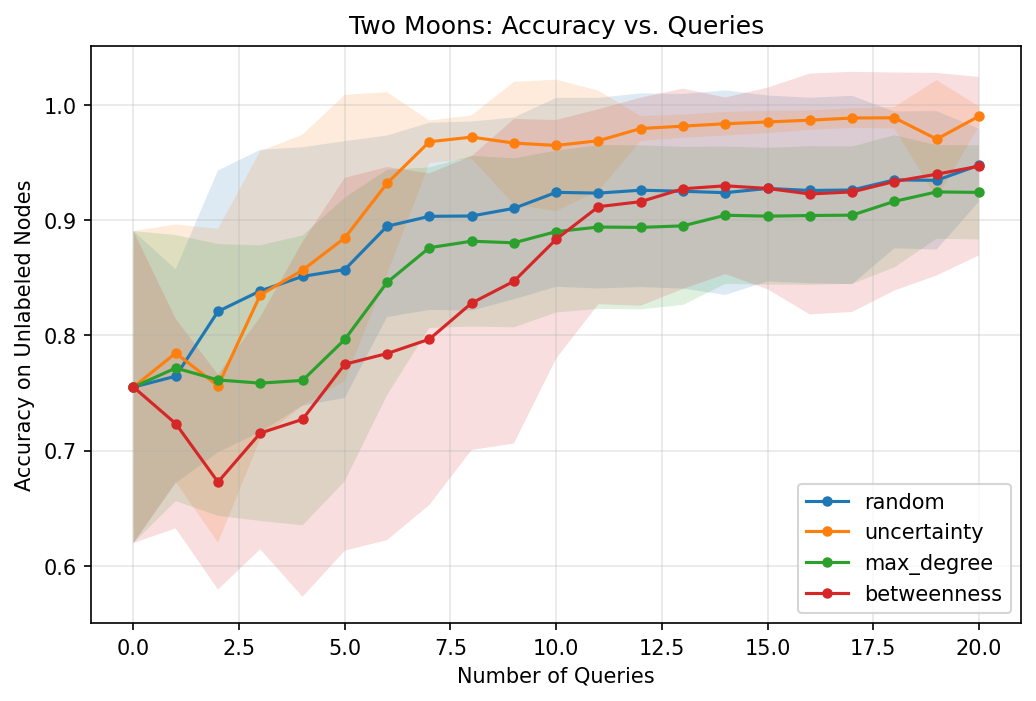
\includegraphics[width=0.85\textwidth]{figures/two_moons_results.png}
\caption{Two Moons: accuracy vs.\ number of queries for each strategy. Uncertainty sampling \cite{Lewis1994} converges fastest, reaching approximately 99\% accuracy by query 12. Random selection improves steadily but more slowly. Maximum degree selection lags behind both alternatives. Betweenness centrality \cite{Freeman1977} performs comparably to random selection. Shaded regions indicate $\pm 1$ standard deviation across 20 trials.}
\label{fig:two_moons}
\end{figure}

\begin{figure}[H]
\centering
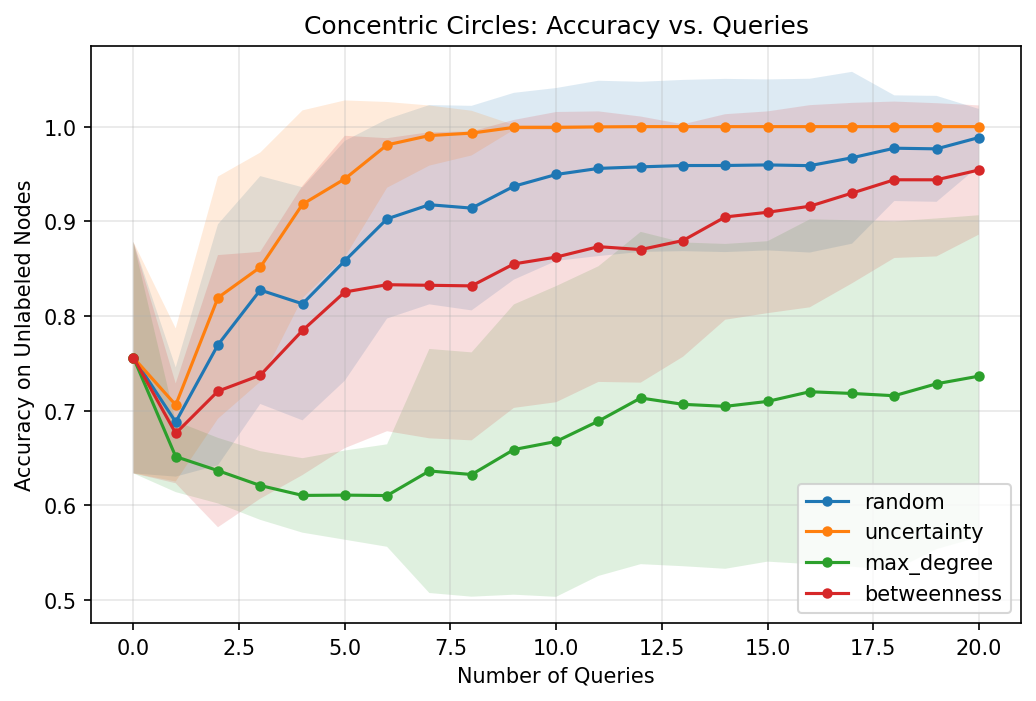
\includegraphics[width=0.85\textwidth]{figures/concentric_circles_results.png}
\caption{Concentric Circles: accuracy vs.\ number of queries. The gap between strategies is especially pronounced. Uncertainty sampling reaches 100\% accuracy by query 12. Maximum degree selection performs dramatically worse than all other strategies, dropping below 75\% accuracy because the highest-degree nodes sit in the densest part of each ring --- far from the radial decision boundary. Betweenness centrality outperforms maximum degree but trails uncertainty sampling.}
\label{fig:circles}
\end{figure}

\begin{figure}[H]
\centering
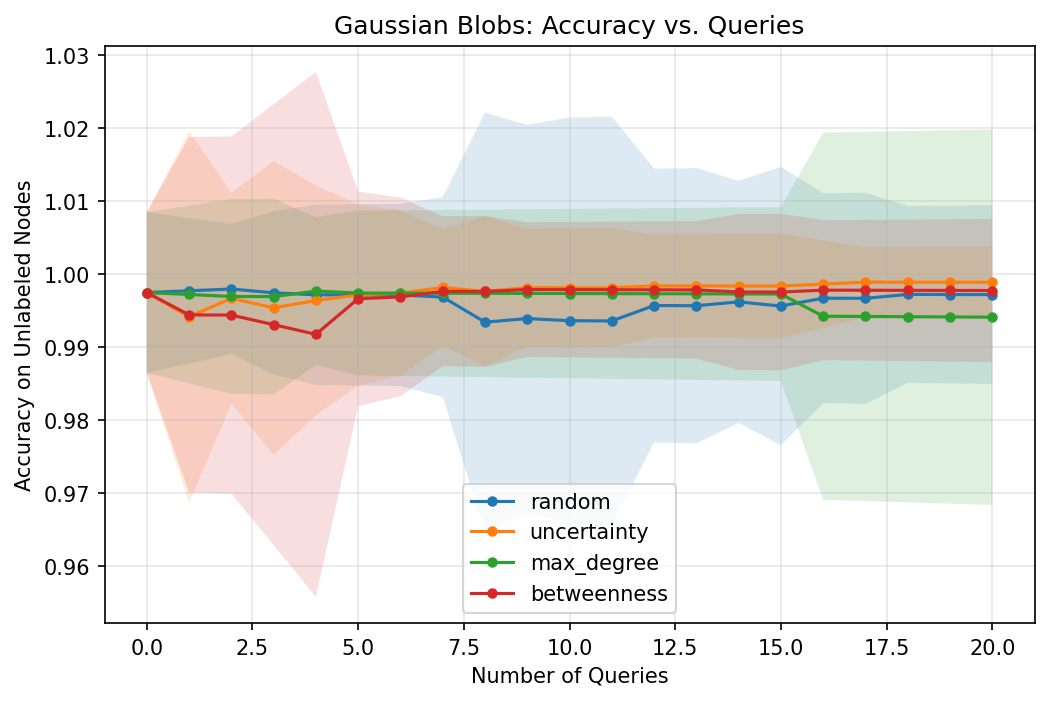
\includegraphics[width=0.85\textwidth]{figures/gaussian_blobs_results.png}
\caption{Gaussian Blobs: accuracy vs.\ number of queries. All strategies achieve near-perfect accuracy almost immediately. With well-separated clusters, GFHF \cite{Zhu2003} classifies correctly using just the two initial seed labels, confirming that strategy choice only matters when the classification problem is genuinely difficult.}
\label{fig:blobs}
\end{figure}

\subsubsection{Two Moons Analysis}

On the two moons dataset (Figure~\ref{fig:two_moons}), uncertainty sampling \cite{Lewis1994} clearly outperforms all alternatives, reaching approximately 99\% accuracy by query~12 while random selection plateaus around 95\% and maximum degree around 92\%. The two moons dataset has a curved, non-convex decision boundary, and uncertainty sampling effectively targets nodes along this boundary where the harmonic function value is close to 0.5 \cite{Zhu2003}. Maximum degree selection picks well-connected nodes that tend to be deep inside one of the moons --- regions already classified correctly --- yielding little new information.

Betweenness centrality \cite{Freeman1977} performs slightly below random on this dataset (94.66\% vs.\ 94.75\%). While bridge nodes are structurally important, the two moons dataset has a relatively uniform density within each moon, meaning betweenness centrality does not consistently identify boundary nodes.

\subsubsection{Concentric Circles Analysis}

The concentric circles dataset (Figure~\ref{fig:circles}) produces the most dramatic differences between strategies. Uncertainty sampling reaches perfect accuracy by query~12. Maximum degree selection, in stark contrast, achieves only 73.65\% --- performing far worse than random selection's 98.85\%. The highest-degree nodes in concentric circles lie in the densest part of each ring, far from the radial boundary between the inner and outer circles. Labeling these nodes wastes the labeling budget on regions where GFHF already propagates labels effectively \cite{Zhu2003}.

Betweenness centrality performs well on this dataset (95.42\%), outperforming maximum degree by a wide margin. In the concentric circles geometry, nodes that bridge the inner and outer rings tend to have high betweenness, aligning better with the decision boundary than high-degree nodes.

\subsubsection{Gaussian Blobs Analysis}

On Gaussian blobs (Figure~\ref{fig:blobs}), all strategies converge to near-perfect accuracy almost immediately. With well-separated Gaussian clusters, the $k$-nearest-neighbor graph has strong within-cluster connections and near-zero between-cluster connections \cite{Zhu2005}. GFHF correctly classifies virtually all nodes with just the two initial seed labels, making additional queries largely redundant regardless of strategy. This result serves as a sanity check confirming that the implementation is correct.

\subsubsection{Summary of Strategy Rankings}

The strategy rankings across datasets reveal a consistent pattern. Uncertainty sampling \cite{Lewis1994} is the best strategy on every dataset, confirming that targeting nodes where the model is most uncertain is the most effective use of a limited labeling budget. Maximum degree selection is consistently the \textit{worst} strategy on datasets with non-trivial decision boundaries, performing worse than even random selection. This is a significant finding: structural importance (as measured by weighted degree) does not correlate with informativeness for label propagation. Betweenness centrality \cite{Freeman1977} falls between random and uncertainty sampling, providing modest benefits from structural information without the drawbacks of degree-based selection.

\subsection{Impact of Label Noise}

Table~\ref{tab:noise_summary} shows how all four strategies degrade under increasing label noise on the two moons dataset. Figures~\ref{fig:noise_uncertainty} and~\ref{fig:noise_random} show the learning curves under noise for uncertainty sampling and random selection, respectively.

\begin{table}[ht]
\centering
\begin{tabular}{lcccc}
\toprule
\textbf{Noise Rate} & \textbf{Random} & \textbf{Uncertainty} & \textbf{Max Degree} & \textbf{Betweenness} \\
\midrule
0\%  & 94.75\% & \textbf{98.99\%} & 92.39\% & 94.66\% \\
5\%  & 93.43\% & \textbf{95.76\%} & 91.18\% & 91.71\% \\
10\% & 89.89\% & \textbf{95.65\%} & 88.76\% & 88.54\% \\
20\% & 83.93\% & \textbf{93.09\%} & 83.85\% & 80.17\% \\
\bottomrule
\end{tabular}
\caption{Mean classification accuracy after 20 queries on the Two Moons dataset under varying noise rates, averaged over 20 trials. Noise is modeled as symmetric label flipping \cite{Fang2014}.}
\label{tab:noise_summary}
\end{table}

\begin{figure}[H]
\centering
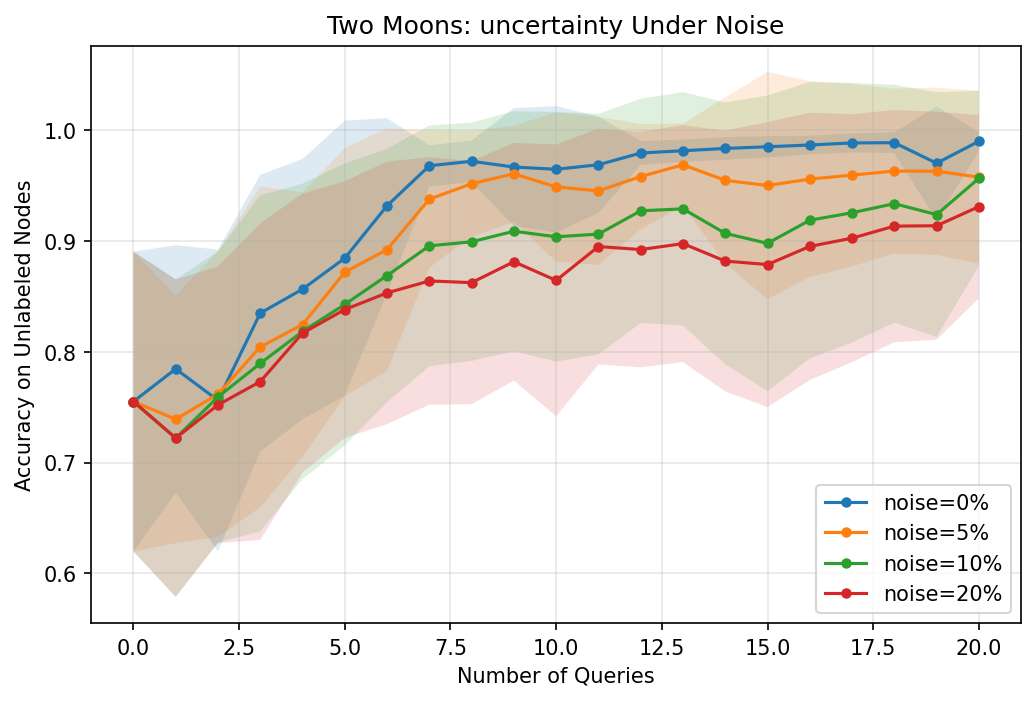
\includegraphics[width=0.85\textwidth]{figures/two_moons_noise_uncertainty.png}
\caption{Two Moons: uncertainty sampling \cite{Lewis1994} under increasing noise rates. At 0\% noise, accuracy reaches approximately 99\% after 20 queries. At 20\% noise, accuracy still reaches approximately 93\%, but convergence is slower and the curve is less stable. Shaded regions show $\pm 1$ standard deviation.}
\label{fig:noise_uncertainty}
\end{figure}

\begin{figure}[H]
\centering
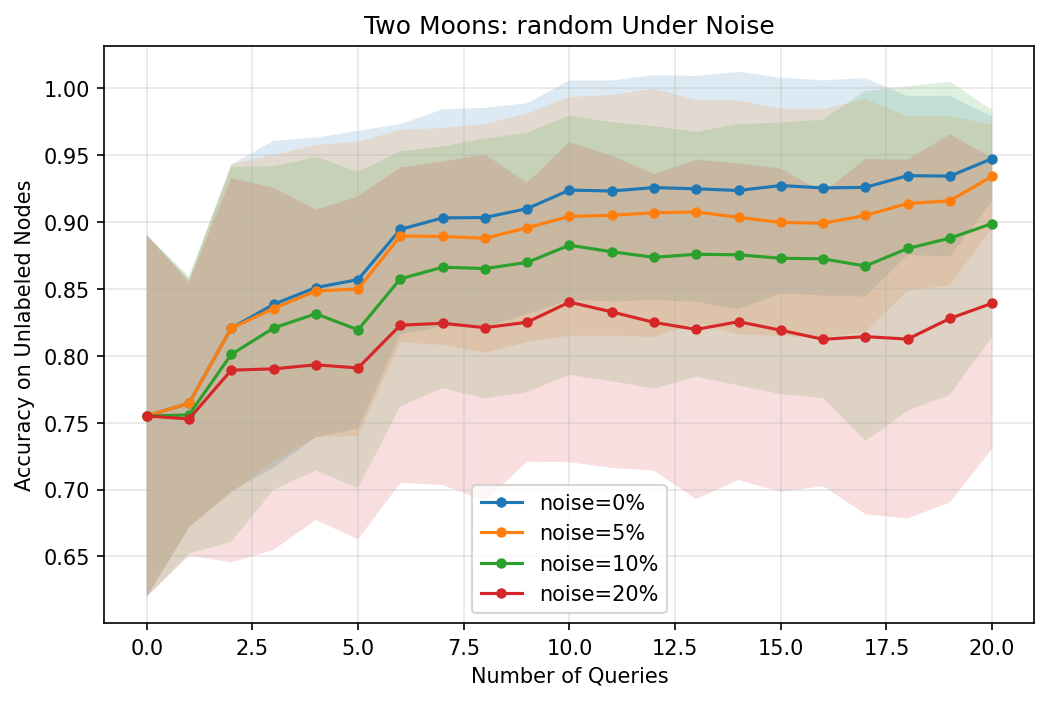
\includegraphics[width=0.85\textwidth]{figures/two_moons_noise_random.png}
\caption{Two Moons: random selection under increasing noise rates. The degradation from 0\% noise (94.75\%) to 20\% noise (83.93\%) is approximately 11 percentage points --- roughly double the degradation experienced by uncertainty sampling over the same range. Shaded regions show $\pm 1$ standard deviation.}
\label{fig:noise_random}
\end{figure}

\subsubsection{Noise Robustness of Uncertainty Sampling}

Several observations emerge from the noise experiments. First, uncertainty sampling \cite{Lewis1994} maintains its advantage over all other strategies at every noise level tested. Even at 20\% noise --- where one in five queried labels is incorrect --- uncertainty sampling achieves 93.09\%, compared to 83.93\% for random and 83.85\% for maximum degree.

Second, the degradation is gradual rather than catastrophic. Moving from 0\% to 20\% noise reduces uncertainty sampling's final accuracy by approximately 6 percentage points (from 98.99\% to 93.09\%), while random selection loses approximately 11 percentage points (from 94.75\% to 83.93\%). This suggests that uncertainty sampling is not only more accurate but also more \textit{robust} to label noise.

\subsubsection{Vulnerability of Boundary Nodes to Noise}

Third, incorrect labels are particularly damaging when they land on structurally important nodes. Because uncertainty sampling selects nodes at the decision boundary, a flipped label at the boundary can mislead predictions for nearby nodes on both sides \cite{Zhu2003}. Despite this vulnerability, uncertainty sampling still outperforms all alternatives, indicating that the benefit of targeting informative nodes outweighs the risk of occasional label corruption.

\subsubsection{Betweenness Centrality Under Noise}

Betweenness centrality shows notable vulnerability to noise. At 0\% noise it performs comparably to random selection (94.66\% vs.\ 94.75\%), but at 20\% noise it degrades to 80.17\% --- worse than all other strategies. Bridge nodes, by definition, connect different regions of the graph \cite{Freeman1977}. When a bridge node receives an incorrect label, the error propagates across the bridge into multiple graph regions, amplifying the damage. This makes betweenness centrality a poor choice in noisy labeling environments.

\subsection{Computational Considerations}

The four strategies differ substantially in computational cost. Let $n$ be the number of nodes and $k$ the number of nearest neighbors.

\begin{itemize}
\item \textbf{Random selection}: $O(1)$ per query (select uniformly at random).
\item \textbf{Uncertainty sampling}: $O(n)$ per query (compute entropy for each unlabeled node using the already-computed harmonic function values).
\item \textbf{Maximum degree}: $O(n)$ per query (sum weights for each unlabeled node; can be precomputed once in $O(nk)$).
\item \textbf{Betweenness centrality}: $O(n^2 \log n + nm)$ per query using Brandes' algorithm \cite{Brandes2001}, where $m$ is the number of edges. For our experiments with $n = 200$ and a $k$-nearest-neighbor graph, this requires approximately 1.6 seconds per query, compared to negligible time for the other strategies.
\end{itemize}

Across 20 queries and 20 trials, uncertainty sampling and maximum degree each complete in under 10 seconds per dataset, while betweenness centrality requires approximately 10 minutes per dataset. For larger graphs, betweenness centrality would become impractical without approximation algorithms \cite{Brandes2001}. Given that betweenness centrality does not outperform the much cheaper uncertainty sampling on any dataset or noise level, the computational overhead is not justified.


%==============================================================================
\section{Discussion}
%==============================================================================

\subsection{Why Uncertainty Sampling Works}

The success of uncertainty sampling \cite{Lewis1994} can be understood through the lens of the GFHF energy functional \cite{Zhu2003}. The harmonic function produces predicted values close to 0.5 precisely at nodes where the label information from both classes is roughly balanced --- that is, at the decision boundary. By labeling these boundary nodes, uncertainty sampling directly resolves the ambiguity that causes the most classification errors.

This insight connects to a broader principle in active learning: the most informative instances to label are those that partition the version space most evenly \cite{Settles2012}. In the graph setting, the ``version space'' is implicitly defined by the smoothness energy, and boundary nodes are exactly those that constrain the energy landscape most strongly.

\subsection{Why Maximum Degree Fails}

Maximum degree selection fails because it conflates \textit{influence} with \textit{informativeness}. A high-degree node has many connections and therefore influences the GFHF predictions of many other nodes \cite{Zhu2003}. However, high-degree nodes tend to sit in the densest part of a cluster, where the harmonic function already assigns confident (near-0 or near-1) predictions. Labeling such a node confirms what GFHF already ``knows'' and wastes the labeling budget.

This failure is especially pronounced on the concentric circles dataset, where the highest-degree nodes sit in the middle of each ring. The decision boundary between the inner and outer circles is a region of \textit{lower} density (the gap between rings), so degree-based selection systematically avoids the most informative nodes.

\subsection{The Role of Graph Geometry}

The datasets in this study were chosen to represent different geometric challenges. Two moons has a \textit{curved, non-convex} boundary that cannot be captured by a linear classifier. Concentric circles has a \textit{radial} boundary where the inner and outer classes have a clear spatial structure. Gaussian blobs have a \textit{linear} boundary between well-separated clusters.

The GFHF method handles all three geometries effectively when given sufficient labels \cite{Zhu2003}, because the Gaussian kernel combined with $k$-nearest-neighbor sparsification captures local structure regardless of the global geometry. However, the active learning strategies respond differently to each geometry. Uncertainty sampling is geometry-agnostic: it always targets the current decision boundary, regardless of its shape. Degree-based and betweenness-based strategies are sensitive to the density distribution, which may or may not align with the decision boundary.

\subsection{Implications for Practitioners}

These results suggest several practical recommendations for researchers and practitioners using graph-based label propagation:

\begin{enumerate}
\item \textbf{Use uncertainty sampling as the default active learning strategy.} It is consistently the best-performing strategy across all datasets and noise levels tested, and its computational cost is negligible compared to the GFHF solve itself.

\item \textbf{Avoid degree-based selection for label propagation.} Despite its intuitive appeal, selecting high-degree nodes wastes the labeling budget on nodes that are already well-classified. This finding is consistent with the broader observation that structural centrality does not imply informativeness \cite{Settles2012}.

\item \textbf{Be cautious with structural heuristics in noisy environments.} Betweenness centrality performs reasonably in noise-free settings but degrades rapidly under label noise because errors at bridge nodes propagate across graph regions.

\item \textbf{Budget allocation matters.} Even a small labeling budget ($B = 20$ queries out of 200 nodes) is sufficient for uncertainty sampling to achieve near-perfect accuracy on datasets with clear cluster structure, demonstrating the efficiency of informed query selection.
\end{enumerate}


%==============================================================================
\section{Conclusion}
%==============================================================================

This project evaluated how active learning query strategies affect the performance of graph-based label propagation using the Gaussian Fields and Harmonic Functions (GFHF) method \cite{Zhu2003}. Four strategies were compared --- random selection, uncertainty sampling \cite{Lewis1994}, maximum degree selection, and betweenness centrality \cite{Freeman1977} --- across three synthetic datasets and under four noise levels.

The results clearly demonstrate that the choice of which nodes to label matters significantly. Uncertainty sampling consistently outperformed all other strategies across every dataset and noise condition. On the two moons dataset, uncertainty sampling reached 98.99\% accuracy after 20 queries, compared to 94.75\% for random and 92.39\% for maximum degree. On concentric circles, uncertainty sampling achieved perfect classification while maximum degree achieved only 73.65\%, highlighting that structural importance (high degree) does not correlate with informativeness for label propagation.

Maximum degree selection performed worse than random selection on every dataset with a non-trivial decision boundary. This is a meaningful finding: the most connected nodes are not the most useful nodes to label. High-degree nodes tend to sit in dense cluster interiors where GFHF already propagates labels effectively \cite{Zhu2003}. The most valuable nodes to label are those at the boundary between classes, where the harmonic function is most uncertain.

Betweenness centrality \cite{Freeman1977} offered modest improvements over maximum degree but did not match uncertainty sampling. More critically, betweenness centrality proved highly vulnerable to label noise, degrading to 80.17\% accuracy at 20\% noise --- worse than all other strategies. The computational cost of betweenness centrality ($O(n^2 \log n)$ via Brandes' algorithm \cite{Brandes2001}) further limits its practical applicability.

The noise experiments confirmed that uncertainty sampling degrades gracefully under imperfect labeling. Even at a 20\% noise rate, uncertainty sampling maintained a clear advantage, losing approximately 6 percentage points compared to 11 for random selection. This robustness is encouraging for real-world applications where label quality cannot be guaranteed \cite{Fang2014}.

Several directions remain for future work. First, implementing Class Mass Normalization \cite{Zhu2003} could improve performance on imbalanced datasets where the simple 0.5 threshold produces biased predictions. Second, more sophisticated noise models --- such as the multi-labeler framework of Fang et al.\ \cite{Fang2014} --- could better simulate realistic crowdsourcing scenarios. Third, combining uncertainty with structural information, as in Bilgic et al.'s ALFNET algorithm \cite{Bilgic2010}, may yield strategies that outperform either approach alone. Finally, evaluating on real-world graph datasets such as citation networks \cite{Bilgic2010} would test whether these findings generalize beyond synthetic settings.


%==============================================================================
% References
%==============================================================================

\begin{thebibliography}{99}

\bibitem{Brandes2001}
U.~Brandes.
\newblock A faster algorithm for betweenness centrality.
\newblock \emph{Journal of Mathematical Sociology}, 25(2):163--177, 2001.

\bibitem{Bilgic2010}
M.~Bilgic, L.~Mihalkova, and L.~Getoor.
\newblock Active learning for networked data.
\newblock In \emph{Proceedings of the 27th International Conference on Machine Learning (ICML-10)}, pages 79--86, Haifa, Israel, 2010.

\bibitem{Chapelle2006}
O.~Chapelle, B.~Sch\"{o}lkopf, and A.~Zien, editors.
\newblock \emph{Semi-Supervised Learning}.
\newblock MIT Press, Cambridge, MA, 2006.

\bibitem{Diestel2017}
R.~Diestel.
\newblock \emph{Graph Theory}.
\newblock Springer, 5th edition, 2017.

\bibitem{Fang2014}
M.~Fang, J.~Yin, and D.~Tao.
\newblock Active learning for crowdsourcing using knowledge transfer.
\newblock In \emph{Proceedings of the 28th AAAI Conference on Artificial Intelligence}, pages 1809--1815, 2014.

\bibitem{Freeman1977}
L.~C.~Freeman.
\newblock A set of measures of centrality based on betweenness.
\newblock \emph{Sociometry}, 40(1):35--41, 1977.

\bibitem{Harris2020}
C.~R.~Harris, K.~J.~Millman, S.~J.~van~der~Walt, et~al.
\newblock Array programming with {NumPy}.
\newblock \emph{Nature}, 585(7825):357--362, 2020.

\bibitem{Lewis1994}
D.~D.~Lewis and W.~A.~Gale.
\newblock A sequential algorithm for training text classifiers.
\newblock In \emph{Proceedings of the 17th Annual International ACM SIGIR Conference on Research and Development in Information Retrieval}, pages 3--12, 1994.

\bibitem{Pedregosa2011}
F.~Pedregosa, G.~Varoquaux, A.~Gramfort, et~al.
\newblock Scikit-learn: Machine learning in {Python}.
\newblock \emph{Journal of Machine Learning Research}, 12:2825--2830, 2011.

\bibitem{Settles2012}
B.~Settles.
\newblock \emph{Active Learning}.
\newblock Synthesis Lectures on Artificial Intelligence and Machine Learning. Morgan \& Claypool Publishers, 2012.

\bibitem{Zhu2003}
X.~Zhu, Z.~Ghahramani, and J.~D.~Lafferty.
\newblock Semi-supervised learning using {G}aussian fields and harmonic functions.
\newblock In \emph{Proceedings of the 20th International Conference on Machine Learning (ICML-03)}, pages 912--919, Washington, DC, 2003.

\bibitem{Zhu2005}
X.~Zhu.
\newblock Semi-supervised learning literature survey.
\newblock Technical Report 1530, Computer Sciences, University of Wisconsin-Madison, 2005.

\end{thebibliography}

\end{document}
